%!TEX root = ./main.tex

\section{Lightweight Resugaring approach}
\label{sec3}

\subsection{Language setting}

\subsubsection{Grammatical restrictions}
Firstly, the whole language should be restricted to tree-structured disjoint expression.

\begin{Def}[disjoint]
For every sub-expression in a expression, its reduction rule is decided by itself.
\end{Def}

This restriction limits the scope of language. Every sub-expression must have no side effect. We will discuss more on side effect in section \ref{mark:side}.

\begin{Def}[tree-structured]
The grammar of the whole language is defined as follow.
\[
\begin{array}{rcl}
\mbox{Exp} &::=& (\mbox{Headid}~\mbox{Exp}*)\\
&|& \mbox{Value}\\
&|& \mbox{Variable}
\end{array}
\]
\end{Def}

The grammatical restrictions give our language a similiar property as church-rosser theorem\cite{churchrosser} for lambda calculus. 

\subsubsection{Context restrictions}
For expressions in CoreLang, the context rules should restrict it to have only one reduction path. The context rules can limit the order of evaluation. This restriction is normal, because a program in general-purposed language should have only one execution path.\label{mark:ctx}

For expressions in SurfLang, context rules should allow every sub-expressions reduced. It's the same as full-$\beta$ reduction.

\subsubsection{Restriction of syntactic sugar}
The form of syntactic sugar is as follow.

\fbox{
$(\mbox{Surfid}\;e_{1}\;e_{2}\;\ldots)$ ~→~ $(\mbox{Headid}\; \ldots)$
}

An counter example of this restriction is $(\mbox{Surfid}\;\ldots\;(e1\;e2)\ldots))$ in LHS. It's for simpler algorithm form, and the expression ability of syntactic sugar will not be changed.

\begin{Def}[Unambiguous]
For every syntactic sugar expressions, it can only desugar to one expression in CoreLang.
\end{Def}

\subsubsection{Grammar Description}
In our language setting, we regard SurfLang and CoreLang as a whole language. The whole language is under restrictions above, and its grammar is defined as follow.

\begin{centering}
	\framebox[38em][c]{
		\parbox[t]{38em}{
			\[
			\begin{array}{rcl}
			\mbox{Exp} &::=& \mbox{DisplayableExp}\\
			&|& \mbox{UndisplayableExp}\\
			\end{array}
			\]
			\[
			\begin{array}{rcl}
			\mbox{DisplayableExp} &::=& \mbox{Surfexp}\\
			&|& \mbox{Commonexp}
			\end{array}
			\]

			\[
			\begin{array}{rcl}
			\mbox{UndisplayableExp} &::=& \mbox{Coreexp}\\
			&|& \mbox{OtherSurfexp}\\
			&|& \mbox{OtherCommonexp}
			\end{array}
			\]
			
			\[
			\begin{array}{rcl}
			\mbox{Coreexp} &::=& (\mbox{CoreHead}~\mbox{Exp}*)
			\end{array}
			\]
			
			\[
			\begin{array}{rcl}
			\mbox{Surfexp} &::=& (\mbox{SurfHead}~\mbox{DisplayableExp}*)
			\end{array}
			\]
			
			\[
			\begin{array}{rcl}
			\mbox{Commonexp} &::=& (\mbox{CommonHead}~\mbox{DisplayableExp}*)\\
			&|& \mbox{Value}\\
			&|& \mbox{Variable}
			\end{array}
			\]
			
			\[
			\begin{array}{rcl}
			\mbox{OtherSurfexp} &::=& (\mbox{SurfHead}~\mbox{Exp}*~\mbox{UndisplayableExp}~\mbox{Exp}*)
			\end{array}
			\]
			
			\[
			\begin{array}{rcl}
			\mbox{OtherCommonexp} &::=& (\mbox{CommonHead}~\mbox{Exp}*~\mbox{UndisplayableExp}~\mbox{Exp}*)
			\end{array}
			\]
		}
	}
\end{centering}

The difference between CoreLang and SurfLang is identified by $Headid$. But there are some terms in CoreLang should be displayed during evaluation, or we need some terms to help us getting better resugaring sequences. So we defined {\bfseries Commonexp}, which origin from CoreLang, but can be displayed in resugaring sequences. The {\bfseries Coreexp} terms are terms with undisplayable CoreLang's Headid. The {\bfseries Surfexp} terms are terms with SurfLang's Headid and all sub-expressions are displayable. The {\bfseries Commonexp} terms are terms with displayable CoreLang's Headid, together with displayable sub-expressions. There exists some other expression during our resugaring process. They have Headid which can be displayed, but one or more subexpressions can't. They are UndisplayableExp.

Take some terms in CoreLang as examples. 

\begin{flushleft}
\begin{tabularx}{\textwidth}%
{|>{\setlength{\hsize}{.4\hsize}\centering\arraybackslash}X  |>{\setlength{\hsize}{1.6\hsize}\centering\arraybackslash}X|}
%{|*{2}{>{\centering\arraybackslash}X|}}
\hline
Syntax & Reduction rules \\ \hline
(if e e e) &\qquad\qquad\qquad(if \#t e2 e3) $\rightarrow$ e2 \newline ~(if \#f e2 e3) $\rightarrow$ e3\\ \hline
(($\lambda$ (x ...) e) e ...) & (($\lambda$ (x0 x1 ...) e) v0 v1 ...) $\rightarrow$ (let ((x0 v0) (($\lambda$ (x1 ...) e) v1 ...))\\ \hline
(($\lambda_N$ (x ...) e) e ...) & (($\lambda_N$ (x0 x1 ...) e) e0 e1 ...) $\rightarrow$ (let ((x0 e0) (($\lambda_N$ (x1 ...) e) e1 ...))\\ \hline
(let ((x e) ...) e) & (let ((x0 e0) (x1 e1) ...) e) $\rightarrow$ (let ((x1 e1) ...) (subst x0 e0 e))\newline (let () e) $\rightarrow$ e\\ \hline
(first e) & (first (list v1 v2 ...)) $\rightarrow$ v1\\ \hline
(rest e) & (rest (list v1 v2 ...)) $\rightarrow$ (list v2 ...)\\ \hline
(empty e) & \qquad\qquad\qquad(empty (list)) $\rightarrow$ \#t \newline (empty (list v1 ...)) $\rightarrow$ \#f\\ \hline
(cons e e) & (cons v1 (list v2 ...)) $\rightarrow$ (list v1 v2 ...)\\ \hline
(op e e) \newline op=+-*/><== & (op v1 v2) $\rightarrow$ arithmetic result\\ \hline
\end{tabularx}
\end{flushleft}

We let {\bfseries if}, {\bfseries let}, {\bfseries $\lambda _{N}$}, {\bfseries empty}, {\bfseries first}, {\bfseries rest} as Coreexp's Headid, {\bfseries Op}, {\bfseries $\lambda$}, {\bfseries cons} as Commonexp's Headid. Then we could show some useful intermediate steps.


\subsection{Algorithm defination}

Our lightweight resugaring algorithm is based on a core algorithm core-algo. For every expression during resugaring process, it may have one or more reduction rules. The core algorithm core-algo chooses the one that satisfies three properties of resugaring, then applies it on the given expression. The core algorithm core-algo is defined as \ref{alg:f}.
\begin{algorithm}
	\caption{Core-algorithm core-algo}
	\label{alg:f}     % 给算法一个标签,以便其它地方引用该算法
	\begin{algorithmic}[1]       % 数字 "1" 表示为算法显示行号的时候,每几行显示一个行号,如:"1" 表示每行都显示行号,"2" 表示每两行显示一个行号,也是为了方便其它地方的引用
		\REQUIRE ~~\\      % 算法的输入参数说明部分
		Any expression $Exp$=$(Headid~Subexp_{1}~\ldots~Subexp_{\ldots})$ which satisfies Language setting
		\ENSURE ~~\\     % 算法的输出说明
		$Exp'$ reduced from $Exp$, s.t. the reduction satisfies three properties of resugaring
		\STATE     Let $ListofExp'$ = $\{Exp'_{1}\;,Exp'_{2}~\ldots\}$
		\IF {$Exp$ is Coreexp or  Commonexp or OtherCommonexp}
		\IF {Lengthof($ListofExp'$)==0}
		\RETURN null; \hfill Case1
		\ELSIF {Lengthof($ListofExp'$)==1}
		\RETURN first($ListofExp'$); \hfill Case2
		\ELSE 
		\RETURN $Exp'_{i}$ = $(Headid~Subexp_{1}~\ldots~Subexp'_{i}~\ldots)$; //where i is the index of subexp which have to be reduced. \hfill Case3
		\ENDIF
		\ELSE 
		\IF {$Exp$ have to be desugared}
		\RETURN desugarsurf($Exp$); \hfill Case4
		\ELSE
		\STATE Let $DesugarExp$ = desugarsurf(Exp)
		\IF {$Subexp_{i}$ is reduced to $Subexp'_{i}$ during $f(DesugarExp)$}
		\RETURN $Exp'_{i}$ = $(Headid~Subexp_{1}~\ldots~Subexp'_{i}~\ldots)$; \hfill Case5
		\ELSE
		\RETURN $DesugarExp$; \hfill Case6
		\ENDIF
		\ENDIF
		\ENDIF
		
	\end{algorithmic}
\end{algorithm}

We briefly describe the core algorithm core-algo in words.

For Exp in language defined as last section, try all reduction rules in the language, get a list of possible expressions ListofExp'=\{$Exp'_{1}$,$Exp'_{2}$,$\ldots$\}. 

Line 2-9 deal with the case when Exp has a CoreLang's Headid. When Exp is value or variable (line 3-4), ListofExp' won't have any element (not reducible). When Exp is of Coreexp or Commonexp (line 5-6, due to the context restriction of CoreLang, only one reduction rule can be applied. When Exp is OtherCommonexp (line 7-8), due to the context restriction of CoreLang, only one sub-expression can be reduced, then just apply core algorithm recursively on the sub-expression.

Line 10-21 deal with the case then Exp has a SurfLang's Headid. When Exp only has one reduction rule (line 11-12), the syntactic sugar has to desugar. If not, we should expand outermost sugar and find the sub-expression which should be reduced (line 14-16), or the sugar has to desugar (line 17-18).


Then, our lightweight-resugaring algorithm is defined as \ref{alg:lwresugar}.

\begin{algorithm}
	\caption{Lightweight-resugaring}
	\label{alg:lwresugar}     % 给算法一个标签,以便其它地方引用该算法
	\begin{algorithmic}[1]       % 数字 "1" 表示为算法显示行号的时候,每几行显示一个行号,如:"1" 表示每行都显示行号,"2" 表示每两行显示一个行号,也是为了方便其它地方的引用
		\REQUIRE ~~\\      % 算法的输入参数说明部分
		Surfexp $Exp$
		\ENSURE ~~\\     % 算法的输出说明
		$Exp$'s evaluation sequences within DSL
		\WHILE {$tmpExp$ = f($Exp$)}
		\IF {$tmpExp$ is empty}
		\RETURN
		\ELSIF {$tmpExp$ is Surfexp or Commonexp}
		\PRINT $tmpExp$;
		\STATE Lightweight-resugaring($tmpExp$);
		\ELSE 
		\STATE Lightweight-resugaring($tmpExp$);
		\ENDIF
		\ENDWHILE
		
	\end{algorithmic}
\end{algorithm}

The whole process of the lightweight resugaring executes core algorithm core-algo, and output sequences which is of Surfexp or Commonexp.

\subsection{Proof of correctness}

First of all, because the difference between our lightweight resugaring algorithm and the existing one is that we only desugar the syntactic sugar when needed, and in the existing approach, all syntactic sugar desugars firstly and then executes on CoreLang.

Second, to prove convenience, define some terms.

$Exp~=~(Headid\;Subexp_{1}\;Subexp_{\ldots} \ldots)$ is any reducible expression in our language.

If we use the reduction rule that desugar Exp's outermost syntactic sugar, then the reduction process is called {\bfseries Outer Reduction}.

If the reduction rule we use reduce $Subexp_{i}$, where $Subexp_{i}$ is $(Headid_{i}~Subexp_{i1}~Subexp_{i\ldots} \ldots)$
\begin{itemize}
	\item If the reduction process is Outer Reduction of $Subexp_{i}$ = $(Headid_{i}~Subexp_{i1}~Subexp_{i\ldots} \ldots)$, then it is called {\bfseries Surface Reduction}.
	\item If the reduction process reduces $Subexp_{ij}$, then it is called {\bfseries Inner Reduction}.
\end{itemize}

{\bfseries Example:}

$(\mbox{if}\; \#t\; Exp_{1}\; Exp_{2})$ → $Exp1$ \hfill Outer Reduction

$(\mbox{if}\; (\mbox{And}\; \#t\; \#f)\; Exp_{1}\; Exp_{2})$ → $(\mbox{if}\; (\mbox{if}\; \#t\; \#f\; \#f)\; Exp_{1}\; Exp_{2})$ \hfill Surface Reduction

$(\mbox{if}\; (\mbox{And}\; (\mbox{And}\; \#t\; \#t)\; \#t) \; Exp_{1}\; Exp_{2})$ → $(\mbox{if}\; (\mbox{And}\; \#t\; \#t)\; Exp_{1}\; Exp_{2})$ \hfill Inner Reduction

\begin{Def}[Upper and lower expression]
For $Exp$=$(Headid\;Subexp_{1}\;Subexp_{\ldots} \ldots)$, $Exp$ is called {\bfseries upper expression}$,Subexp_{i}$is called {\bfseries lower expression}.
\end{Def}

We only need to prove that all the 6 cases of core algorithm core-algo won't effect its properties. Case 1 and case 3 won't effect any properties, because it does what CoreLang should do.

\begin{proof}[Proof of Emulation]
\hfill\\
For case 4 and 6, desugaring won't change Emulation property, because desugaring and resugaring are interconvertible.

For case 2 and 5, our core algorithm reduces the sub-expression which should be reduced. So if applying core algorithm core-algo on the subexpression satisfies emulation property, then this two cases satisfy. A recursive proof it is.
todo:case5
\end{proof}

\begin{proof}[Proof of Abstraction]
\hfill\\
It's true, because we only display the sequence which satisfies abstraction property.
\end{proof}

\begin{lemma}
If no syntactic sugar desugared before it has to, then coverage property is satisfied.
\end{lemma}

\begin{proof}[Proof of Lemma]
Assume that no syntactic sugar not necessarily expanded desugars too early, existing an expression in CoreLang

$Exp$ = $(Headid\;Subexp_{1}\;Subexp_{\ldots} \ldots)$ which can be resugared to

$ResugarExp'$ = $(Surfid\;Subexp'_{1}\;Subexp'_{\ldots}\ldots)$, and $ResugarExp'$ is not displayed during lightweight-resugaring. Then

\begin{itemize}
	\item Or existing
	
	$ResugarExp$=$(Surfid\;Subexp'_{1}\;\ldots\;Subexp_{i}\;Subexp'_{\ldots}\ldots)$ in resugaring sequences, such that the expression after $ResugarExp$ desugaring reduces to $Exp$, and the reduction reduces $ResugarExp$'s sub-expression $Subexp_{i}$. If so, outermost syntactic sugar of $ResugarExp$ is not expanded. So if $ResugarExp'$ is not displayed, then the sugar not necessarily expanded desugars too early, which is contrary to assumption.
	
	
	\item Or existing
	
	$ResugarExp$=$(Surfid'\;\ldots\;ResugarExp'\;\ldots)$ in resugaring sequences, such that the expression after $ResugarExp$ desugaring reduces to $Exp$, and $Exp$ is desugared from $ResugarExp'$'s sub-expression. If $ResugarExp'$ is not displayed, then the outermost syntactic sugar is expanded early, which is contrary to assumption.
	todo
	%使得$ResugarExp$解糖后得到的表达式单步规约得到$Exp$,且该$Exp$是从$ResugarExp$中的子表达式$ResugarExp'$解糖得到,说明此步单步规约不涉及$ResugarExp'$的规约。而如果不能展示$ResugarExp'$,则说明该语法糖在执行前面的序列被提前破坏了,也与假设矛盾。

\end{itemize}
\end{proof}

\begin{proof}[Proof of Coverage]
\hfill\\
For case 4 and 6, the syntactic sugar has to desugar.

For case 2 and 5, the reduction occurs in sub-expression of $Exp$. So if applying core algorithm core-algo on the subexpression doesn't desugar syntactic sugars not necessarily expanded, then this two cases don't. A recursive proof it is.
\end{proof}

\subsection{Implementation}

Our lightweight resugaring approach  is implemented using PLT Redex\cite{SEwPR}, which is an semantic engineering tool based one reduction semantics\cite{reduction}. The whole framework is as Fig\ref{fig:frame}.

\begin{figure}[h]
	\centering
	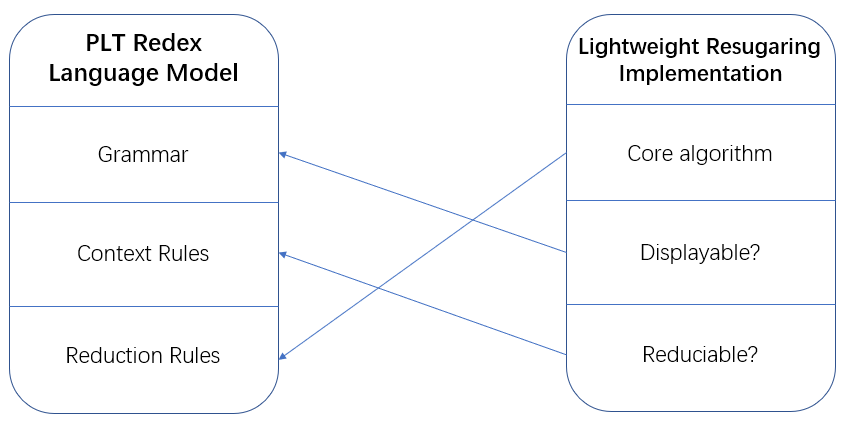
\includegraphics[width=12cm]{images/frame.png}
	\caption{framework of implementation}
	\label{fig:frame}
\end{figure}

The grammar of the whole language contains Coreexp, Surfexp and Commonexp as the language setting in sec\ref{sec3}. OtherSurfexp is of Surfexp and OtherCommonexp is of Commonexp. The identifier of any kind of expression is Headid of expression. If we need to add a syntactic sugar to the whole language, only three steps is needed.

\begin{enumerate}
\item Add grammar of the syntactic sugar.
\item Add context rules of the sugar, such that any sub-expressions can be reduced.
\item Add desugar rules of the sugar to reduction rules of the whole language.
\end{enumerate}

Then inputting an expression of the syntactic sugar to lightweight-resugaring will get the resugaring sequences.

\subsection{Evaluation}
\label{sec6}

We test some applications on the tool implemented using PLT Redex. Note that we set CBV's lambda calculus as terms in commonexp, because we need to output some intermediate sequences including lambda expressions in some examples. It's easy if we want to skip them.

\subsubsection{simple sugar}
\label{mark:simple}

We construct some simple syntactic sugar and try it on our tool. Some sugar is inspired by the first work of resugaring\cite{resugaring}. The result shows that our approach can process all sugar features of their first work.

We take a SKI combinator syntactic sugar as an example. We will show why our approach is lightweight.

\begin{flushleft}
	$S$ $\rightarrow$ $(\lambda _{N}~(x_{1}~x_{2}~x_{3})~(x_{1}~x_{2}~(x_{1}~x_{3})))$
	
	$K$ $\rightarrow$ $(\lambda _{N}~(x_{1}~x_{2})~x_{1})$
	
	$I$ $\rightarrow$ $(\lambda _{N}~(x)~x)$
\end{flushleft}

Althought SKI combinator calculus is a reduced version of lambda calculus, we can construct combinators' sugar based on call-by-need lambda calculus in our CoreLang. For expression

 $(S~(K~(S~I))~K~xx~yy)$, we get the following resugaring sequences as Fig \ref{fig:SKI}.

\begin{figure}[ht]
	\centering
	\parbox[t]{\textwidth}{
				\begin{center}
				{
					\small\selectfont
					(S (K (S I)) K xx yy)\\
					↓\\
					(((K (S I)) xx (K xx)) yy)\\
					↓\\
					(((S I) (K xx)) yy)\\
					↓\\
					(I yy ((K xx) yy))\\
					↓\\
					(yy ((K xx) yy))\\
					↓\\
					(yy xx)
				}
				\end{center}
			}
	\caption{SKI's resugaring sequences}
	\label{fig:SKI}
\end{figure}

For existing approach, the sugar expression should firstly desugar to
\begin{flushleft}
$((\lambda _{N}
   (x_{1} x_{2} x_{3})
   (x_{1} x_{3} (x_{2} x_{3})))
  ((\lambda _{N} (x_{1} x_{2}) x_{1})
   ((\lambda _{N}
     (x_{1} x_{2} x_{3})
     (x_{1} x_{3} (x_{2} x_{3})))
    (\lambda _{N} (x) x)))
  (\lambda _{N} (x_{1} x_{2}) x_{1})
  xx
  yy)$
\end{flushleft}

Then in our CoreLang, the execution of expanded expression will contain 33 steps. For each step, there will be many attempts to match and substitute the syntactic sugars. We will omit more steps for a larger expression. So the unidirectional resugaring algorithm makes our approach lightweight.todo

\subsubsection{hygienic macro}
\label{mark:hygienic}

The second work\cite{hygienic} mainly processes hygienic macro compared to first work. We try a $Let$ sugar , which is a common hygienic sugar example, on our tool. Our algorithm can easily process hygienic macro without special data structure. The $Let$ sugar is define as follow

$(Let\;x\;v\;exp)$ $\rightarrow$ $(Apply\;(\lambda\;(x)\;exp)\;v)$

Take $(Let~x~1~(+~x~(Let~x~2~(+~x~1))))$ for an example. First, a temp expression

$(Apply\;(\lambda\;(x)\;(+~x~(Let~x~2~(+~x~1))))\;1)$

is needed. (case 5 or 6)Then one-step try on the temp expression, we will get

$(+~1~(Let~1~2~(+~1~1)))$ which is out of the whole language's grammar. In this case, it is not a good choice to desugar the outermost $Let$ sugar. Then we just apply the core-algo f on the sub-expression where the error occurs ($(+~x~(Let~x~2~(+~x~1)))$ in this example). So the right intermediate sequence $(Let~x~1~(+~x~3))$ will be get.

In practical application, we think resugaring for a unhygienic rewriting system is not interesting at all, because hygienic macro can be easily processed by rewriting system. So in the finally implementation of our tool, we just use PLT Redex's binding forms to deal with hygienic macros. But we did try it on the version without hygienic rewriting system.

\subsubsection{recursive sugar}
Recursive sugar is a kind of syntactic sugars where call itself or each other during the expanding. For example,

$(Odd\;e)$ $\rightarrow$ $(if\;(>\;e\;0)\;(Even\;(-\;e\;1)\;\#f))$

$(Even\;e)$ $\rightarrow$ $(if\;(>\;e\;0)\;(Odd\;(-\;e\;1)\;\#t))$

are typical recursive sugars. The previous works can process this kind of syntactic sugar easily, because boundary conditions are in the sugar itself.

Take $(Odd~2)$ as an example. The previous work will firstly desugar the expression using the rewriting system. Then the rewriting system will never start resugaring as Fig\ref{fig:odd} shows.

\begin{figure}[ht]
	\centering
	\parbox[t]{\textwidth}{
				\begin{center}
				{
					\small\selectfont
					(Odd 2)\\
					↓\\
					(if (> 2 0) (Even (- 2 1) \#f))\\
					↓\\
					(if (> (- 2 1) 0) (Odd (- (- 2 1) 1) \#t))\\
					↓\\
					(if (> (- (- 2 1) 1) 0) (Even (- (- (- 2 1) 1) 1) \#f))\\
					↓\\
					{\ldots}
				}
				\end{center}
				
			}
	\caption{Odd2's desugaring process}
\label{fig:odd}
\end{figure}

Then the advantage of our approach is embodied. Our lightweight approach doesn't require a whole expanding of sugar expression, which gives the framework chances to judge boundary conditions in sugars themselves, and showing more intermediate sequences. We get the resugaring sequences as Fig \ref{fig:rec} of the former example using our tool.

\begin{figure}[ht]
	\centering
	\parbox[t]{\textwidth}{
				\begin{center}
				{
					\small\selectfont
					(Odd 2)\\
					↓\\
					(Even (- 2 1))\\
					↓\\
					(Even 1)\\
					↓\\
					(Odd (- 1 1))\\
					↓\\
					(Odd 0)\\
					↓\\
					\#f
				}
				\end{center}
				
			}
	\caption{Odd2's resugaring sequences}
\label{fig:rec}
\end{figure}

We also construct some higher-order syntactic sugars and test them. The higher-order feature is important for constructing practical syntactic sugar. And for syntactic sugar's feature, it is of recursive sugar. Giving the following two higher-order syntactic sugar as examples.

\begin{flushleft}
	$(map\;e\;(list\;v_1\ldots))$→
	
	$(if\;(empty\;(list\;v_1\ldots))\;(list)\;(cons\;(e\;(first\;(list\;v_1\ldots)))\;(map\;e\;(rest\;(list\;v_1\ldots)))))$
\end{flushleft}

\begin{flushleft}
	$(filter\;e\;(list\;v_1\;v_2\ldots))$→
	
	$(if\;(e\;v_1)\;(cons\;v_1\;(filter\;e\;(list\;v_2\ldots)))\;(filter\;e\;(list\;v_2\ldots)))$
	
	$(filter\;e\;(list))$ → $(list)$
\end{flushleft}
These two syntactic sugars use different sugar forms to implement. For $Map$ sugar, we use if expression in CoreLang to constrain the boundary conditions. For $Filter$ sugar, we use two different parameters' form, which is another easy way for constructing syntactic sugar. The testing results show as Fig\ref{fig:map} \ref{fig:filter}.

\begin{figure}[ht]
	\centering
	\parbox[t]{\textwidth}{
				\begin{center}
				{
					\small\selectfont
					(map (λ (x) (+ 1 x)) (list 1 2 3))\\
					↓\\
					(cons 2 (map (λ (x) (+ 1 x)) (list 2 3)))\\
					↓\\
					(cons 2 (cons 3 (map (λ (x) (+ 1 x)) (list 3))))\\
					↓\\
					(cons 2 (cons 3 (cons 4 (map (λ (x) (+ 1 x)) (list)))))\\
					↓\\
					(cons 2 (cons 3 (cons 4 (list))))\\
					↓\\
					(cons 2 (cons 3 (list 4)))\\
					↓\\
					(cons 2 (list 3 4))\\
					↓\\
					(list 2 3 4)
				}
				\end{center}
				
			}
	\caption{Map's resugaring sequences}
\label{fig:map}
\end{figure}

\begin{figure}[ht]
	\centering
	\parbox[t]{\textwidth}{
	
				\begin{center}
				{
					\small\selectfont
					(filter (λ (x) (and (> x 3) (< x 6))) (list 1 2 3 4 5 6 7))\\
					↓\\
					(filter (λ (x) (and (> x 3) (< x 6))) (list 2 3 4 5 6 7))\\
					↓\\
					(filter (λ (x) (and (> x 3) (< x 6))) (list 3 4 5 6 7))\\
					↓\\
					(filter (λ (x) (and (> x 3) (< x 6))) (list 4 5 6 7))\\
					↓\\
					(cons 4 (filter (λ (x) (and (> x 3) (< x 6))) (list 5 6 7)))\\
					↓\\
					(cons 4 (cons 5 (filter (λ (x) (and (> x 3) (< x 6))) (list 6 7))))\\
					↓\\
					(cons 4 (cons 5 (filter (λ (x) (and (> x 3) (< x 6))) (list 7))))\\
					↓\\
					(cons 4 (cons 5 (filter (λ (x) (and (> x 3) (< x 6))) (list))))\\
					↓\\
					(cons 4 (cons 5 (list)))\\
					↓\\
					(cons 4 (list 5))\\
					↓\\
					(list 4 5)
				}
					
				\end{center}
				
			}
	\caption{Filter's resugaring sequences}
\label{fig:filter}
\end{figure}
\subsection{Compare to previous work}

As mentioned many times before, the biggest difference between previous resugaring approach and our approach, is that our approach doesn't need to desugar the sugar expresssion totally. Thus, our approach has the following advantages compared to previous work.

\begin{itemize}
	\item {\bfseries Lightweight} As the example at sec\ref{mark:simple}, the match and substitution process searchs all intermediate sequences many times. It will cause huge cost for a large program. So out approach---only expanding a syntactic sugar when necessarily, is a lightweight approach.
	\item {\bfseries Friendly to hygienic macro} Previous hygienic resugaring approach use a new data structure---abstract syntax DAG, to process resugaring of hygienic macros. Our approach simply finds hygienic error after expansion, and gets the correct reduction instead. 
	\item {\bfseries More syntactic sugar features} The ability of processing recursive sugar is a superiority compared to previous work. The key point is that recursive syntactic sugar must handle boundary conditions. Our approach handle them easily by not necessarily desugaring all syntactic sugars. Higher-order functions, as an important feature of functional programming, was supported by many daily programming languages. So the ability on higher-order sugar is important. 
	\item {\bfseries Rewriting rules based on reduction semantics} Any syntactic sugar that can expressed by reduction semantics can be used in our approach. It will give more possible forms for constructing syntactic sugars. todo:example?
\end{itemize}